\begin{frame}
\frametitle{Learning network protocols despite imperfect assumptions}
\begin{centering}
Can we learn a protocol with imperfect asumptions about the number of bottlenecks?
\end{centering}
\end{frame}

\begin{frame}
\frametitle{Imperfect assumptions about the number of bottlenecks}
\large
\begin{centering}

\begin{itemize}
\item<2-> What if we train on a one-bottleneck topology\\
\begin{centering}
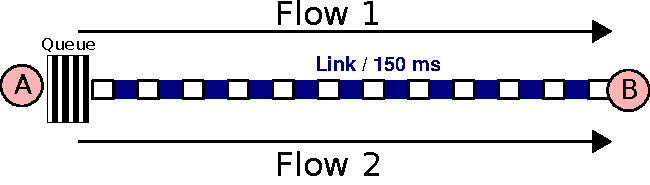
\includegraphics[width=0.8\textwidth]{onelink.pdf}
\end{centering}
\item<3-> But, test on a two-bottleneck topology\\
\begin{centering}
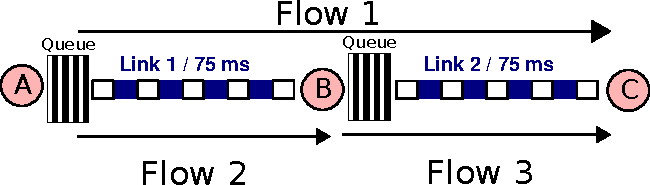
\includegraphics[width=0.8 \textwidth]{twolink.pdf}
\end{centering}
\end{itemize}
\end{centering}
\end{frame}

\begin{frame}
\frametitle{Imperfect assumptions about the number of bottlenecks}
\begin{centering}

\noindent \only<1>{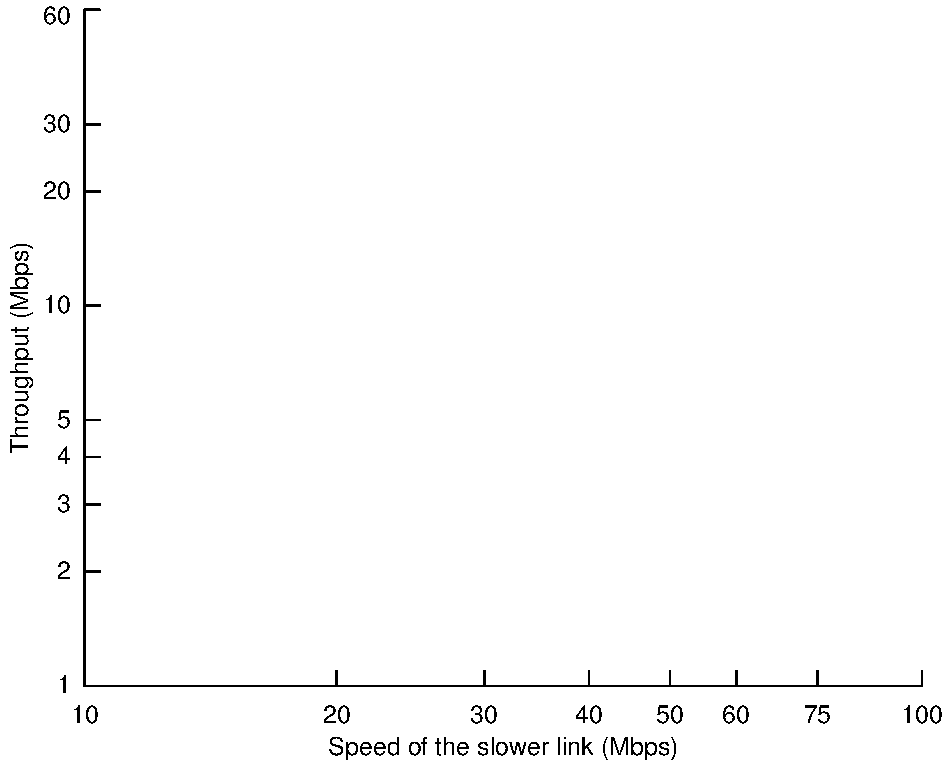
\includegraphics[width=3.4 in]{multilink-background.pdf}}\only<2>{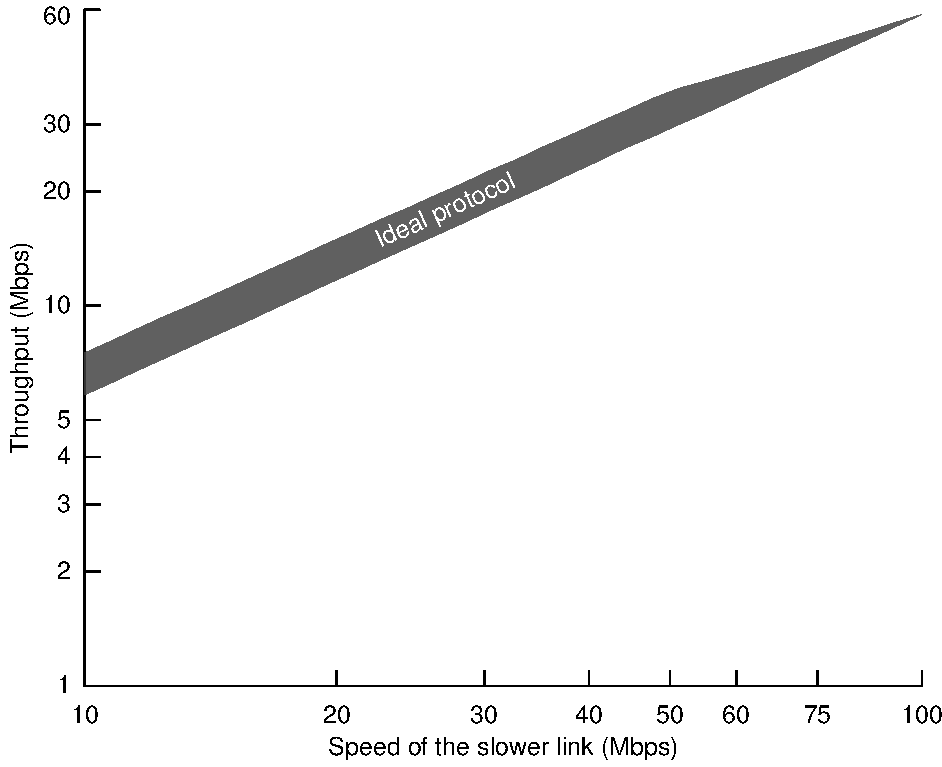
\includegraphics[width=3.4 in]{multilink-omniscient.pdf}}\only<3>{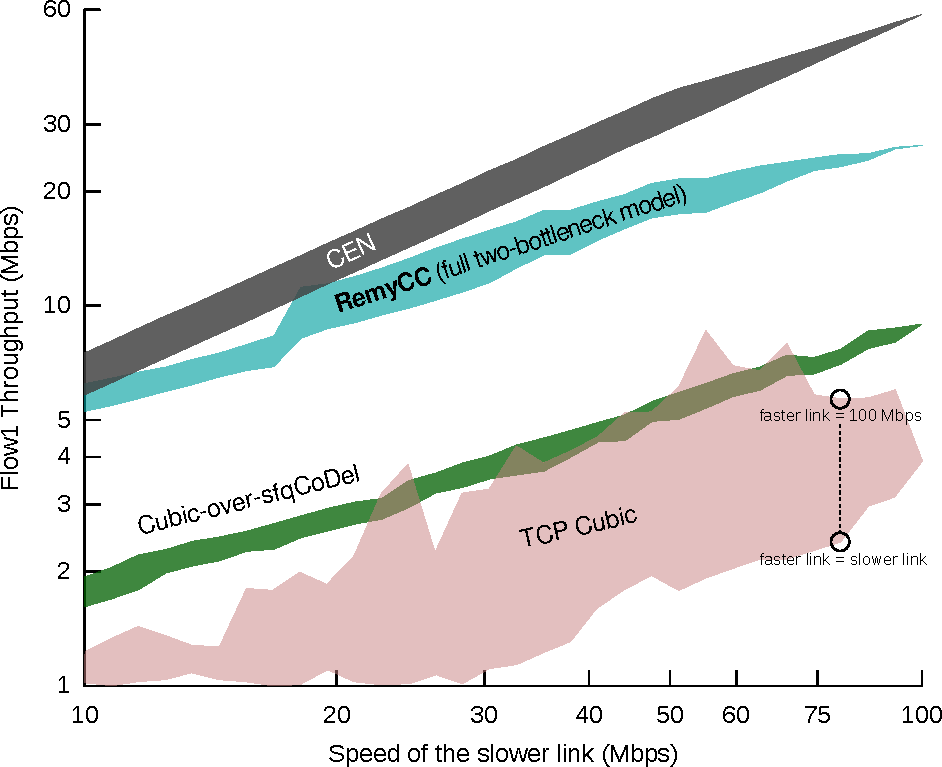
\includegraphics[width=3.4 in]{multilink-twolink.pdf}}\only<4>{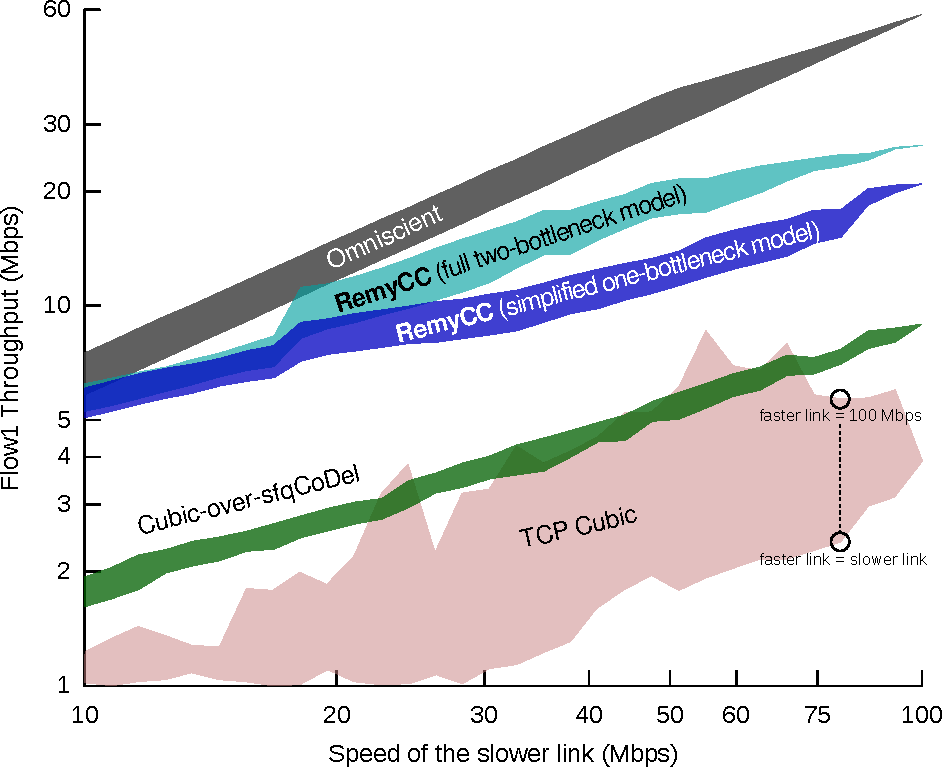
\includegraphics[width=3.4 in]{multilink-onelink.pdf}}\only<5>{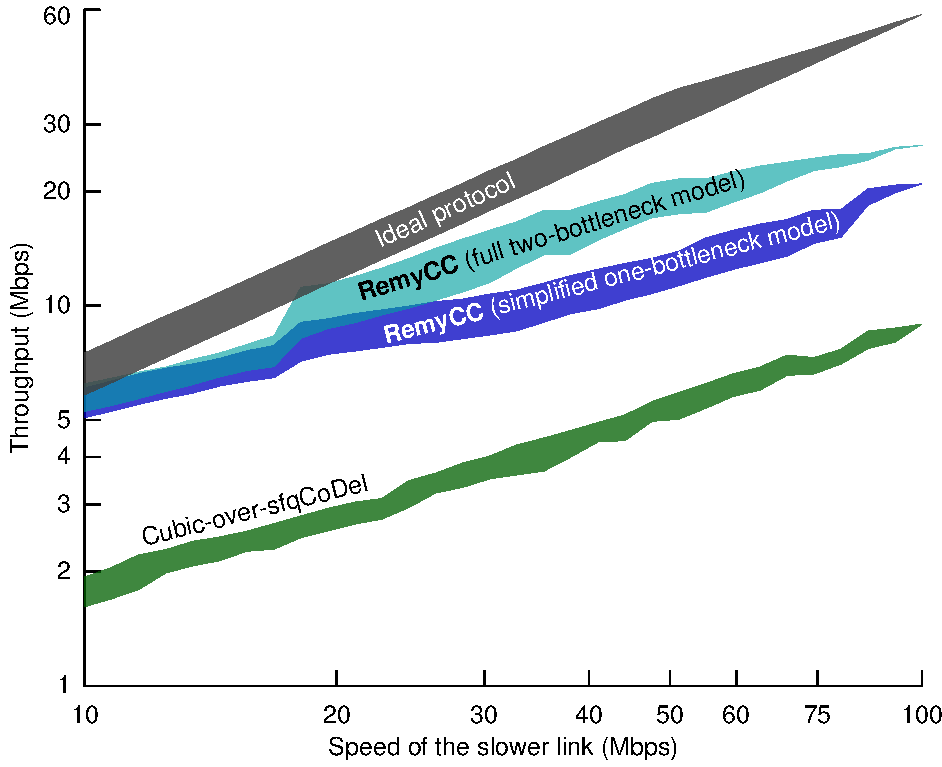
\includegraphics[width=3.4 in]{multilink-rest.pdf}}
\only<7>{Simplifying a two-bottleneck network to a single-bottleneck network only modestly hurts performance}
\end{centering}
\end{frame}

